\section{Elasto-plasticity}

Plasticity is a property of a material to undergo a non-reversible change of shape in response to an applied force. During the elasto-plastic deformation, the onset of plasticity is determined by a yield criterion and post-yield deformation is governed by the yield criterion and a plastic potential. To illustrate features of elasto-plasticity deformation, we consider a uniaxial test of stress depicted in Fig. \ref{fig:uniax_test}.

\begin{figure}[!htb]
  \centering
  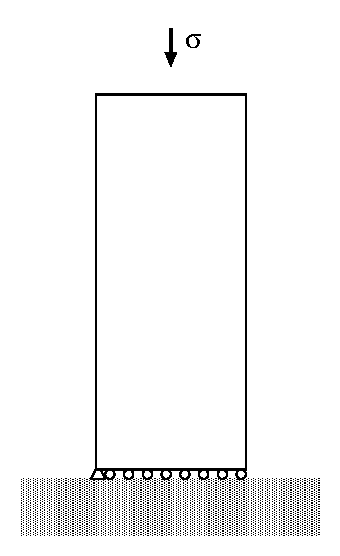
\includegraphics[scale=0.6]{M/figure/uniaxial.eps}
  \caption{Uniaxial test }
  \label{fig:uniax_test}
\end{figure}

This means only one direction has non-zero stress and strain,e.g $\stress=\sigma_{yy}$ and $\strain=\gamma_{yy}$.
Different material exhibits different elasto-plastic behavior. Fig. \ref{fig:uniax_lp} depicts a typical

\begin{figure}[!htb]
  \centering
  \input{M/figure/plast.eepic}
  \caption{Stress-strain curve of 1D problems }
  \label{fig:uniax_lp}
\end{figure}

stress-strain curve of the uniaxial test. If load $\stress$ is gradually increased, a corresponding point in $(\stress, \strain)$ plane are moving from 0 to A. Up to A, stress reaches a value $\Stress_0$, so called yield stress. If the load is removed gradually before its reaches the yield value, the point follows the line from A to 0. On the other hand, if the load is continually increased after stress is bigger than   $\Stress_0$, the material experiences plastic deformation. Assuming the curve is extended from A to B during load acting. If we remove the load gradually, the point  will not take the way its from, i.e. from B to A to 0. On the contrary, it will move from B to C linearly. Furthermore, if the load is applied again, the point will take the path from \mbox{C $\longrightarrow$ B $\longrightarrow$ D}.

This implies that: i) The unloading is elastic and there is still strain $\strain^p$ left after the load being removed,
Therefore, the plastic deformation is irreversible; ii) The strain is admissible to be decomposed into several
components, e.g. $\Stra=\Stra^e+\Stra^p$; iii) The relationship of stress-strain is history dependent curve.  Based on the last point and the  Hook's law, the constitutive equation for the 1D deformation problem can be described as

\begin{eqnarray}
\sigma_{yy}=E\varepsilon_{yy}^e=E(\varepsilon_{yy}-\varepsilon_{yy}^p)
\label{eqn:constitu_M_1D}
\end{eqnarray}

where $E$ is so called Young's modulus. If the stress-strain is monotonic increasing after yielding, the material shows hardening behavior. For some porous media, softening  behavior may be observed and its stress-strain curve looks like what depicted in Fig. \ref{fig:uniax_lp1}.

\begin{figure}[!htb]
  \centering
  \input{M/figure/plastics.eepic}
  \caption{Softening }
  \label{fig:uniax_lp1}
\end{figure}

For the constitutive equation, the case of more than one direction have non-zero stress and strain are much more complicated. A yield function $\yieldf$ and a plastic potential $\plsp$ are introduced to establish a constitutive equation. Normally, the variables of the two functions are the first, second or third stress invariant $\sivi$, $\sivii$ or $\siviii$. If we cast the yield functions to the principal stress space, we get the yield surfaces. Fig. \ref{fig:yieldsfc} depticts three typical yield surfaces of porous media.

\begin{figure}[!htb]
  \begin{center}
   \begin{minipage}[t]{0.48\textwidth}
     \begin{center}
    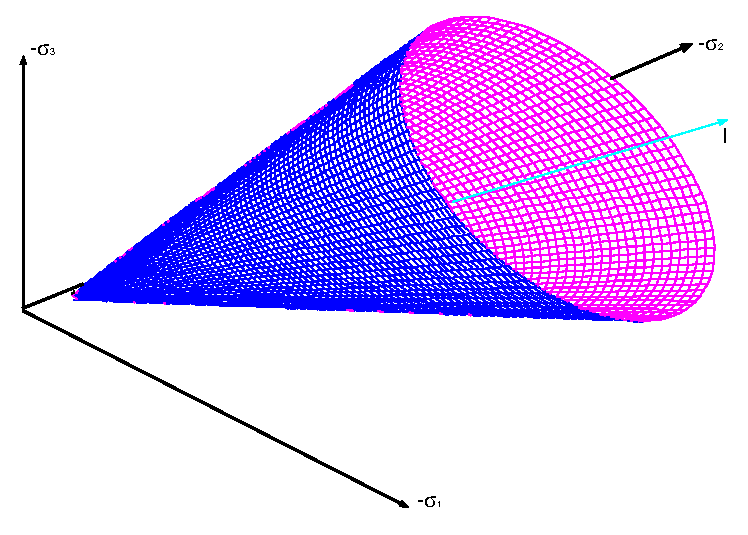
\includegraphics[scale=0.28]{M/figure/yieldsfc_dp.eps}
    \centerline{(Drucker-Prager)}
    \end{center}
   \end{minipage}
   \hspace{0.02\textwidth}
   \begin{minipage}[t]{0.48\textwidth}
    \begin{center}
    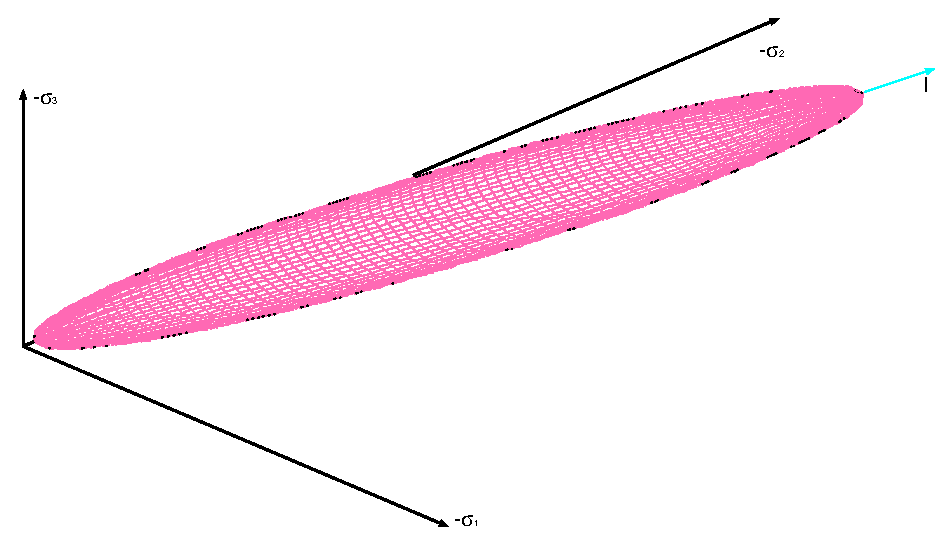
\includegraphics[scale=0.28]{M/figure/yieldsfc_cam.eps}\\
    \centerline{(Cam-Clay)}
    \end{center}
   \end{minipage}\\
   %
   \begin{minipage}[t]{0.48\textwidth}
     \begin{center}
    \includegraphics[scale=0.28]{M/figure/yieldsfc_wm.eps}
    \centerline{(Single yield surface)}
    \end{center}
   \end{minipage}
  \end{center}
  \caption{Yield surface}
  \label{fig:yieldsfc}
\end{figure}

If the stress path of any point locates inside the surface, the point undergoes elastic deformation. Otherwise, the stress status is determined by the Kuhn-Tucker criterion for the loading or unloading:

\begin{eqnarray}
\label{kuhn_tucker}
\quad \dot{\yieldf} \leq 0, \,\, \dot{ \PlasticParameter}\,{\yieldf} = 0,\,\mbox{or},\,  \dot{ \PlasticParameter} \geq 0
\end{eqnarray}

is then used to check the yield status.

Since the stress path in plastic deformation is history dependent, we describe the constitutive equations in the sense of increment of stress and strain.
Considering the generalized Hook's law (\ref{eq:hook}),  the relationship of incremantal stress  tensor $d \Stress$ and incremantal strain tensor $d \Stra$ the relationship of
stress and strain obeys the generalized Hook's law:

\begin{eqnarray}
d\Stress
= {\mathbf D} d\Stra^e=
{\mathbf D} (d\Stra-d\Stra^p)
\label{eq:ghook}
\end{eqnarray}

From the definition of plastic potential surface $\plsp$, and
normality law, it is possible to express the generalized plastic
strain increment if the potential surface is smooth. Since
$d\Stra^p$ lies parallel to the normal to $\plsp$ at $\Stress$, we
may write

\begin{eqnarray}
d\Stra^p =d \PlasticParameter \frac{\partial \plsp}{\partial \Stress}
\label{eqn:flowrule}
\end{eqnarray}

where $d \PlasticParameter$ is non-negative factor, plastic
multiplier. Equaion (\ref{eqn:flowrule}) is so clalled flow rule. Hence, the general elasto-platic constitutive equation is given by

\begin{eqnarray}
d\Stress
= {\mathbf D} d\Stra^e=
{\mathbf D} (d\Stra-d \PlasticParameter \frac{\partial \plsp}{\partial \Stress})
\label{eq:constitu_m}
\end{eqnarray}.

The flow rule is associative if $\yieldf\equiv\plsp$. Otherwise, it is non-associative. Typical plastic models, i.e. yield  functions and plastic potentials are described below.

\textit{Drucker-Prager model}

This model is a function of the two stress invariants and hardening parameter. Its yield function takes the form

\begin{eqnarray}
\yieldf (\Stress, \kappa) =\left\Vert{\devS} \right\Vert+\alpha\sivi-y(\kappa)=0 \\
\plsp (\Stress, \kappa) =\left\Vert{\devS} \right\Vert+\beta \sivi-y(\kappa)=0
\label{eqn:dp}
\end{eqnarray}

where $\alpha$ is a coefficient related to the internal frictional angle, $y(\kappa)$ is the yield stress depending on the hardening parameter.

\textit{Cam-Clay model}

Similar to the Drucker-Prager model, the Cam-Clay model is a funtion of both of the first and the second stress invariants. The generalized Cam-Clay model reads:

\begin{eqnarray}
\yieldf=q^2+M^2\pm(\pm-\pm_{cn})=0
\label{eqn:cc}
\end{eqnarray}

where $q=\sqrt{3/2}=\left\Vert {\devS} \right\Vert$, $\pm=\sivi/3$ the mean stress, $M$ is the slope of the critical state line in a $q-\pm$ digram and $\pm_{cn}$ is the isotropic preconsolidation pressure. The rate of $\pm_{cn}$ is given by

\begin{eqnarray}
{\frac{\mathrm d\, \pm\phantom{^-_-}}{\mathrm d\,  \epsilon^p_v}}=\frac{(1+e)\pm}{\lambda_c-\kappa_c}
\label{eqn:cc_pcn}
\end{eqnarray}

with $e$ the void ratio, $\epsilon^p_v$ the volume plastic strain, $\lambda_c$ the virgin compression index and $\lambda_c$  the swelling/recompression index.

The model also describes the nonlinear elastic behavior of the clay-like media before plastic yielding occurs, in which the bulk modulus $K$ is dependent of stress status as

\begin{eqnarray}
K=\frac{1+e}{\kappa_c}\pm=0
\label{eqn:cc_K}
\end{eqnarray}

with $\mu=3(1-2\nu)K/(2(1+\nu))$.

%-------------------------------------------------------------------------
\subsection{Plastic plate - von Mises plasticity (2D)}

\subsubsection*{Problem definition}

This is a typical plane strain benchmark for von Mises plasticity,
which is defined in \cite{SteEtAl:03}. We first analyze this example
to compare the behavior of two approaches on pure plastic
deformation problems. In the present simulation, a  quarter of plate
is taken due to the symmetry of the problem. The model set-up is
depicted in Fig. \ref{ex1_model}. The radius of the hole is 10$mm$.
Two points as point 1 and point 2 are specified to monitor the
evolution of variables. Point 1 is at  one third of the distance
from point 3 to point 4.

\begin{figure}[!htb]
\centering
    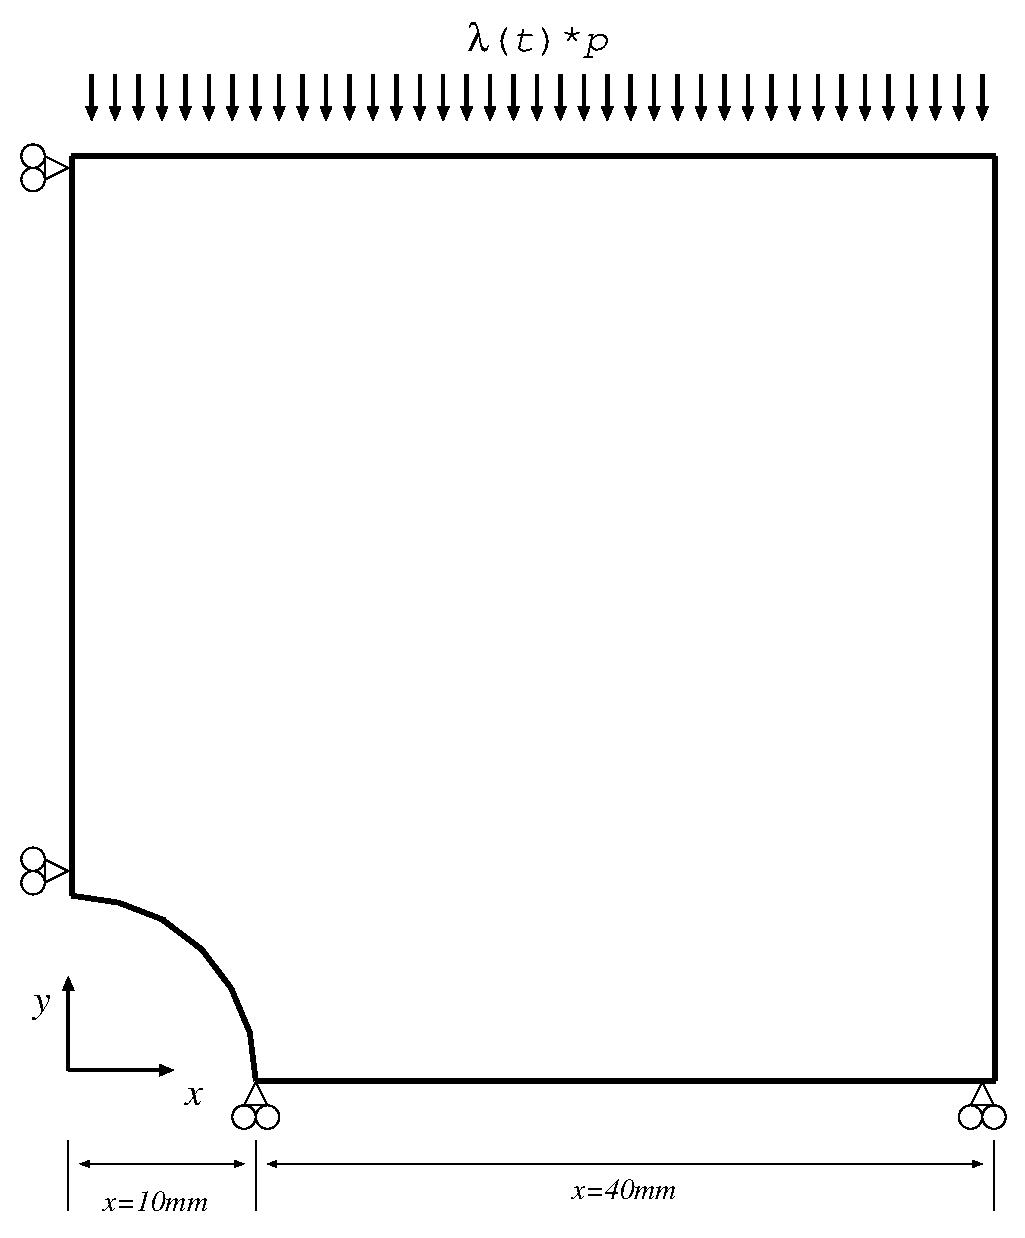
\includegraphics[scale=0.3]{M/ex1_model.eps}\\
   \caption{Stretched steel plate with a hole: one quarter}
  \label{ex1_model}
\end{figure}

\subsubsection*{Boundary conditions}

Traction boundary condition, $p=100N/mm^2\lambda(t)$  is
prescribed on the top with $\lambda(t)$, the time dependent scaling
factor. The case of  cycling loading is investigated with a scaling
function depicted in Fig. \ref{ex1_load}, in which,
$\lambda_{max}=4.1$.

\begin{figure}[!thb]
\centering
    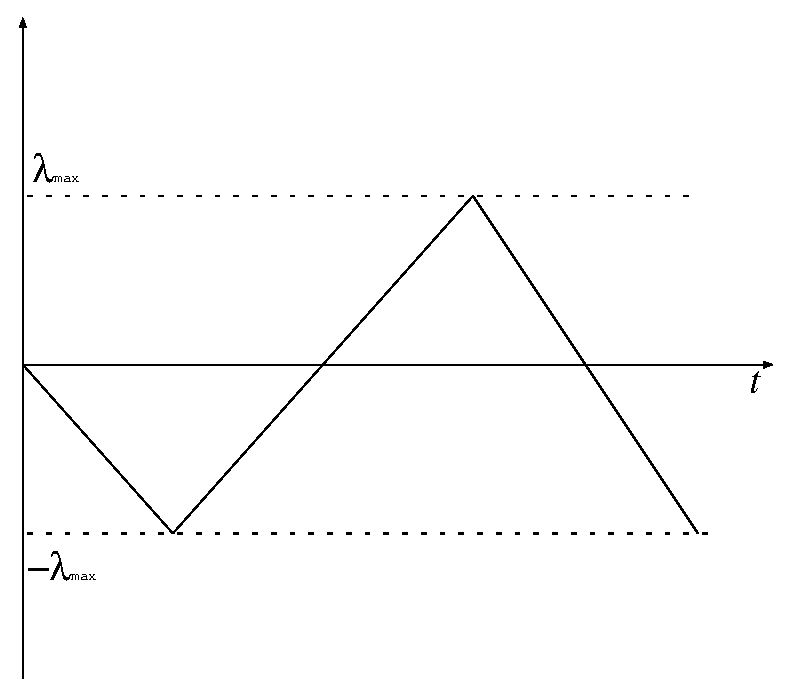
\includegraphics[scale=0.5]{M/ex1_load.eps}\\
   \caption{Time dependent load factor}
  \label{ex1_load}
\end{figure}

The domain is triangulated as depicted in Fig. \ref{ex1_mesh}.

\begin{figure}[!htb]
\centering
    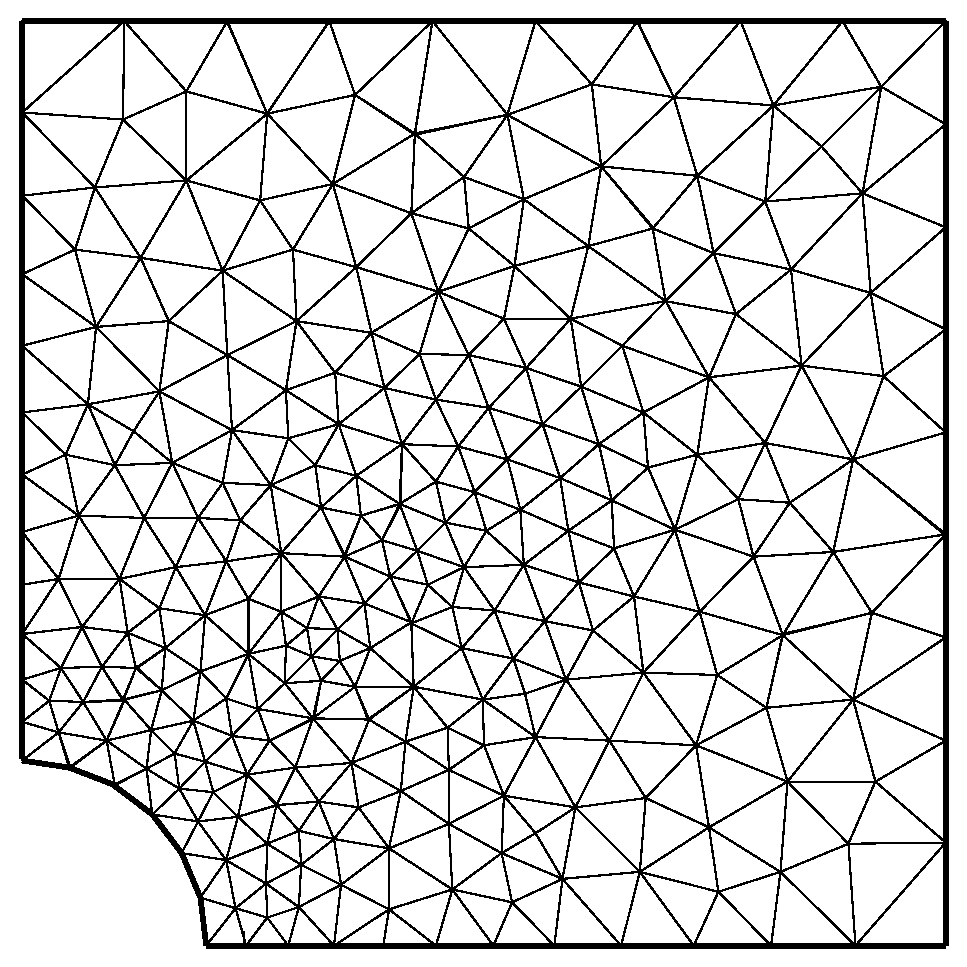
\includegraphics[scale=0.3]{M/ex1_mesh_gfem.eps}\\
   \caption{Mesh: 269 nodes and 484 elements}
  \label{ex1_mesh}
\end{figure}

\subsubsection*{Material properties}

The domain is assumed in homogeneous state. Table \ref{ex1_table1}
gives the material parameters\cite{SteEtAl:03}.

\begin{table}[!thb]
\centering
\caption{Material properties}
\label{ex1_table1}
\begin{tabular}{lll}
\hline\hline\noalign{\smallskip}
Property & Value & Unit \\
\noalign{\smallskip}\hline\noalign{\smallskip}
Young's modulus & $206900$  & $N/mm^2$ \\
Poisson's ratio & $0.29$       & $-$ \\
Initial yield stress & $450$       & $N/mm^2$ \\
Hardening modulus & $0.0$       & $kPa$ \\
\noalign{\smallskip}\hline\hline
\end{tabular}
\end{table}

\subsubsection*{Results}

The loading takes 60 steps with constant increment of
$\lambda_{max}/10$.  The similar distribution of plastic strain and
vertical stain given in Fig.\ref{ex2_cont1} shows implies the
behavior of von Mises plasticity.

%Contour plot
\begin{figure}[!thb]
  \begin{center}
   \begin{minipage}[t]{0.48\textwidth}
     \begin{center}
    \includegraphics[scale=0.28]{M/ex1_pls_4.1.eps}
    \centerline{(Plastic strain)}
    \end{center}
   \end{minipage}
   \hspace{0.02\textwidth}
   \begin{minipage}[t]{0.48\textwidth}
    \begin{center}
    \includegraphics[scale=0.28]{M/ex1_strain_yy_4.1.eps}\\
    \centerline{(Vertical strain)}
    \end{center}
   \end{minipage}\\
   %
  \end{center}
  \caption{Distribution of plastic strain and vertical strain at $\lambda_{max}/10$}
  \label{ex2_cont1}
\end{figure}

The evolution of horizontal displacements at point 1 and point 2
along with periodic load factor $\lambda (t)$ are shown on Fig.

\ref{ex2_loadp}.
\begin{figure}[!htb]
  \begin{center}
   \begin{minipage}[t]{0.48\textwidth}
     \begin{center}
    \includegraphics[scale=0.28]{M/ex1_load_v_ux_p1.eps}
    \centerline{(Point 1)}
    \end{center}
   \end{minipage}
   \hspace{0.02\textwidth}
   \begin{minipage}[t]{0.48\textwidth}
    \begin{center}
    \includegraphics[scale=0.28]{M/ex1_load_v_ux_p2.eps}\\
    \centerline{(Point 2)}
    \end{center}
   \end{minipage}\\
   %
  \end{center}
  \caption{Evolution of horizontal displacement vs load factor}
  \label{ex2_loadp}
\end{figure}

\subsubsection*{Benchmark deposit}
\begin{tabular}{|l|l|l|}
  \hline
  Benchmark & Problem type & Path in benchmark deposit \\
  \hline
 \emph{m\_mises} & M & benchmarks\verb \M\ \\
  \hline
\end{tabular}

%-------------------------------------------------------------------------
\subsection[Plastic plate - Drucker-Prager plasticity (2D)]{Plastic plate - Drucker-Prager plasticity, enhanced strain element (2D)}

\subsubsection*{Problem definition}

In this application, we analyze a plane strain biaxial failure
de\-for\-ma\-tion problem with triangle and quadrilateral
elements, correspondingly. We use an enhanced strain approximation
to simulate the displacement discontinuity after failure appears.
Neighbor relationships of an element object are essential data for
constructing the deforming mesh and to determinate the propagation
orientation of the discontinuity in the failure analysis.

From the view point of bifurcation theory, strain localization is a
bifurcation phenomenon, which takes place when the velocity field
moves away from the branch of continuous solutions and takes a new
path of discontinuous solutions. If standard finite element is
applied to this problem, we have to refine mesh adaptively near the
localization area. Otherwise, the system equation is ill-posed. The
strong discontinuity approach with enhanced strain element avoids
the ill-posed system equations and therefore avoid mesh sensitive of
the analysis \cite{SanWri84}.

The set-up of the biaxial compression problem as proposed by
\cite{Bo00} is shown in Fig. \ref{fig:biaxial}. The geometry of the
specimen is simplified to a rectangle with size of 1m$\times$3m.
\begin{figure}[!htb]
\center
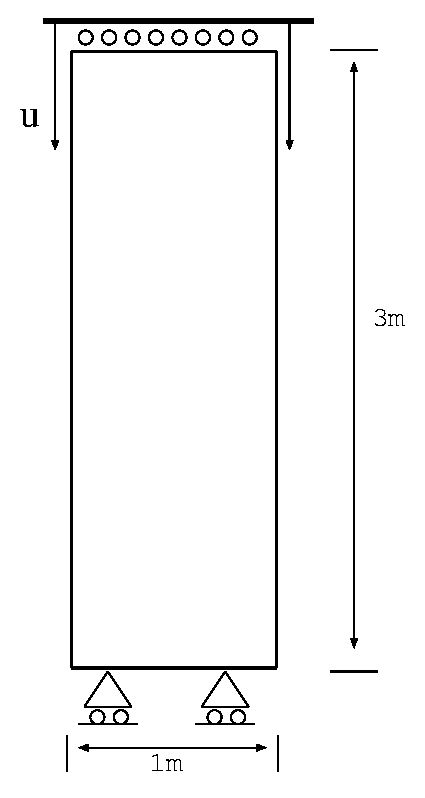
\includegraphics[scale=0.45]{M/biaxial.eps}
\caption{Plane strain biaxial test}
 \label{fig:biaxial}
\end{figure}

\subsubsection*{Boundary conditions}

The bottom of the specimen is placed on horizontal roll supporters.
While the top of it is only allowed to a vertical down movement
$u_z$. Both lateral sides are considered to be traction free.

\subsubsection*{Material properties}

The non-associative flow rule is adopted for the Drucker-Prager model. All material parameters are given in Table (\ref{ex1:tableDP})

\begin{table}[H]
\centering
\begin{tabular}{lll}
\hline \hline
Parameter   &  Unit  & Value\\
\hline
  Young's modulus &  $kPa$ &  $2\times10^4$ \\
\hline\hline
  Poisson ratio & - &  0.4 \\
\hline
  Parameter $\alpha$  & - & 0.233345 (30$^\circ$ friction angle)\\
\hline
  Parameter $\beta$  & - &  0.141421 (16.53$^\circ$ dilatancy angle)\\
\hline
  Initial stress $\sigma_0$ & $kPa$ &  29.69 (20 of initial cohesion)\\
\hline
  Hardening modulus $H$ & $kPa$ &  100\\
\hline
  Localized softening modulus $H_{\delta}$ & $kPa$ & -1000, varying\\
\hline \hline
\end{tabular}
\caption{Material parameters of the plane strain biaxial test}
\label{ex1:tableDP}
\end{table}

\subsubsection*{Results}
Fig. \ref{fig:loc} shows the deformed sample exhibiting localization. Fig. \ref{fig:vreact} depicts the stress
reaction at the top surface due to the displacement load. The results agrees with what given in \cite{Bo00}

\begin{figure}[H]
\begin{center}
\includegraphics[scale=0.35]{M/m_sdc.eps}
\end{center}
\caption{Vertical reaction of the top}.
 \label{fig:loc}
\end{figure}
\begin{figure}[H]
\begin{center}
\includegraphics[scale=0.35]{M/m_sdc_s_u.eps}
\end{center}
\caption{Vertical reaction of the top}.
 \label{fig:vreact}
\end{figure}

\subsubsection*{Benchmark deposit}
\begin{tabular}{|l|l|l|}
  \hline
  Benchmark & Problem type & Path in benchmark deposit \\
  \hline
 \emph{m\_sdc} & M & benchmarks\verb \M\ \\
  \hline
\end{tabular}


%-------------------------------------------------------------------------
\subsection{Plastic plate - Cam-Clay plasticity (2D)}
\label{sec:ccup}

\subsubsection*{Problem definition}

This example is generally applied to verify a critical state plastic
mode, i.e. Cam-Clay model. We consider a quarter of the cylindrical
sample of 5cm in diameter and 10cm in length.

\subsubsection*{Initial and Boundary conditions}

The bottom surface is roller supported.
A vertical down displacement is prescribed to make an axial strain of 50\%. The movement in the radial
direction on the top surface is allowed. The cylindrical  surface is traction free.

\subsubsection*{Material properties}

Table \ref{tab:m_cc_s} shows the material parameters.
 \begin{table}[H]
\begin{tabular}{lrl}
\hline\noalign{\smallskip}
  \hline
 Meaning & Value & Unit \\
  \hline
 Poisson ratio & $0.3$ & ---\\
 Slope of the critical state line & $1.2$ & ---\\
 Virgin compression index & $0.2$ & ---\\
 swelling/recompression index & $0.02$ & ---\\
 Initial preconsolidation pressure & $60.0$ & $--$\\
 Initial void ratio & $1.5$ & $--$\\
 \hline\hline
\end{tabular}
\caption{Solid material properties} %\footnotesize
\label{tab:m_cc_s}
\end{table}

\subsubsection*{Results}

The problem is axisymmetrical. A relationship between von Mises type stress, the second stress invariant, and the axial strain is illustrated in Fig. \ref{fig:m_cc_s_r}. The results agrees with what given in \cite{SheSloYu00}.

\begin{figure}[H]
  \begin{center}
    \includegraphics[scale=0.3]{M/cc_s_s_e.eps}
  \end{center}
  \caption{Axial strain vs von Mises type stress }
  \label{fig:m_cc_s_r}
\end{figure}

\subsubsection*{Benchmark deposit}

\begin{tabular}{|l|l|l|}
  \hline
  Benchmark & Problem type & Path in benchmark deposit \\
  \hline
 \emph{m\_cc\_quad\_s}\&  \emph{m\_cc\_tri\_s}& M & benchmarks\verb \M\ \\
  \hline
\end{tabular}


%-------------------------------------------------------------------------
\subsection{Plastic plate - Rotational hardening plasticity (2D)}

\subsubsection*{Problem definition}

This example is a plane strain compression test on a
material with both isotropic and rotational hardening behaviour.

The geometry of the specimen used is $0.34$~m height and $0.1$~m
width. We denote by $\sigma_x$ the stress acting on the both
lateral sides of the specimen and by $\sigma_y$ the stress applied
to the top side of the specimen.
 The set-up of the problem is shown in Fig.~\ref{fig:ssy}.

\begin{figure}[H]
\center
\includegraphics[scale=0.3]{M/ssy_mesh.eps}
\caption{Plane strain biaxial test: rotational hardening}
 \label{fig:ssy}
\end{figure}

A vertical down displacement load is applied on the top boundary.

\subsubsection*{Material properties}

Assume all initial stresses are zero. The material properties of the rotational hardening model
are defined in Table \ref{Tab_par_oedo}
\begin{table}[!htb]
\centering
\begin{tabular}{lll}
\hline \hline
Parameter   &  Unit  & Value\\
\hline
  Young's modulus &  Pa &  1e+08 \\
\hline
  Poisson ratio & - &  0.3 \\
\hline
  $\alpha_0$       &  -        & 0.0 \\
  $\beta_0$        &  -        & 0.26 \\
  $\delta_0$       &  $m^2/N$  & 3.5e-07\\
  $ \varepsilon_0$ &  $m^2/N$  & 1.0e-7\\
  $\kappa_0$       &  $N/m^2$  & 0.0  \\
  $\gamma_0$       &  -        & 0.0 \\
  $m_0$            &  -        & 0.569 \\
\hline
  $\hat {\alpha}$  &  -        & 0.0 \\
  $\hat {\beta_0}$ &  -        & 0.29\\
  $\hat{\delta_0}$ &  $m^2/N$  & 8.81e-9\\
  $\hat{\varepsilon_0}$&  $m^2/N$  & 1.5e-8 \\
  $\hat{\kappa_0}$ &  $N/m^2$  & 0.0  \\
  $\hat{\gamma_0}$ &  -        & 0.0 \\
  $\hat{m_0}$      &  -        & 1.0 \\
\hline
  $\psi_1$         &   -       & 0.55\\
  $\psi_2$         &  -        & -0.26\\
\hline
  $C_h$            &  -        & 0.81e-3\\
  $C_d$            &  -        & 0.60e-3\\
\hline
  $b_r$            &  -        & 100.0\\
  $m_r$            &  -        & -3.0\\
\hline \hline
\end{tabular}
\caption{\label{Tab_par_oedo}Material parameters of rotational hardening
model }
\end{table}

\subsubsection*{Results}

The output of the results in a
specified point, i.e, a center of a finite element close to the
geometrical center of the domain (Fig.~\ref{fig:ssy}), is used to analyze the model behavior.
Fig. \ref{fig:ssy_u_s} shows the varying of vertical stress along with vertical displacement at the top boundary.

\begin{figure}[!htb]
\center
\includegraphics[scale=0.4]{M/ssy_u_s.eps}
\caption{Vertical stress vs vertical displacement}
 \label{fig:ssy_u_s}
\end{figure}

\subsubsection*{Benchmark deposit}

\begin{tabular}{|l|l|l|}
  \hline
  Benchmark & Problem type & Path in benchmark deposit \\
  \hline
 \emph{m\_ssy\_quad}& M & benchmarks\verb \M\ \\
  \hline
\end{tabular}


